% appendix.tex
El análisis principal se centra en el crecimiento temporal en función del tamaño de entrada. Sin embargo, para una evaluación integral, a continuación se adjuntan gráficas adicionales correspondientes a la huella de memoria y al comportamiento de los algoritmos bajo tamaños de entrada estáticos.

\subsection*{A.1 Uso de Memoria en Algoritmos de Ordenamiento}
En la Figura \ref{fig:app_mem_sorting} se aprecia que \texttt{std::sort} y Quick Sort (algoritmos in-place) mantienen un consumo de memoria mínimo en comparación con Merge Sort y Patience Sort, cuyo requerimiento espacial crece de forma lineal conforme aumenta $n$.

\begin{figure}[H]
    \centering
    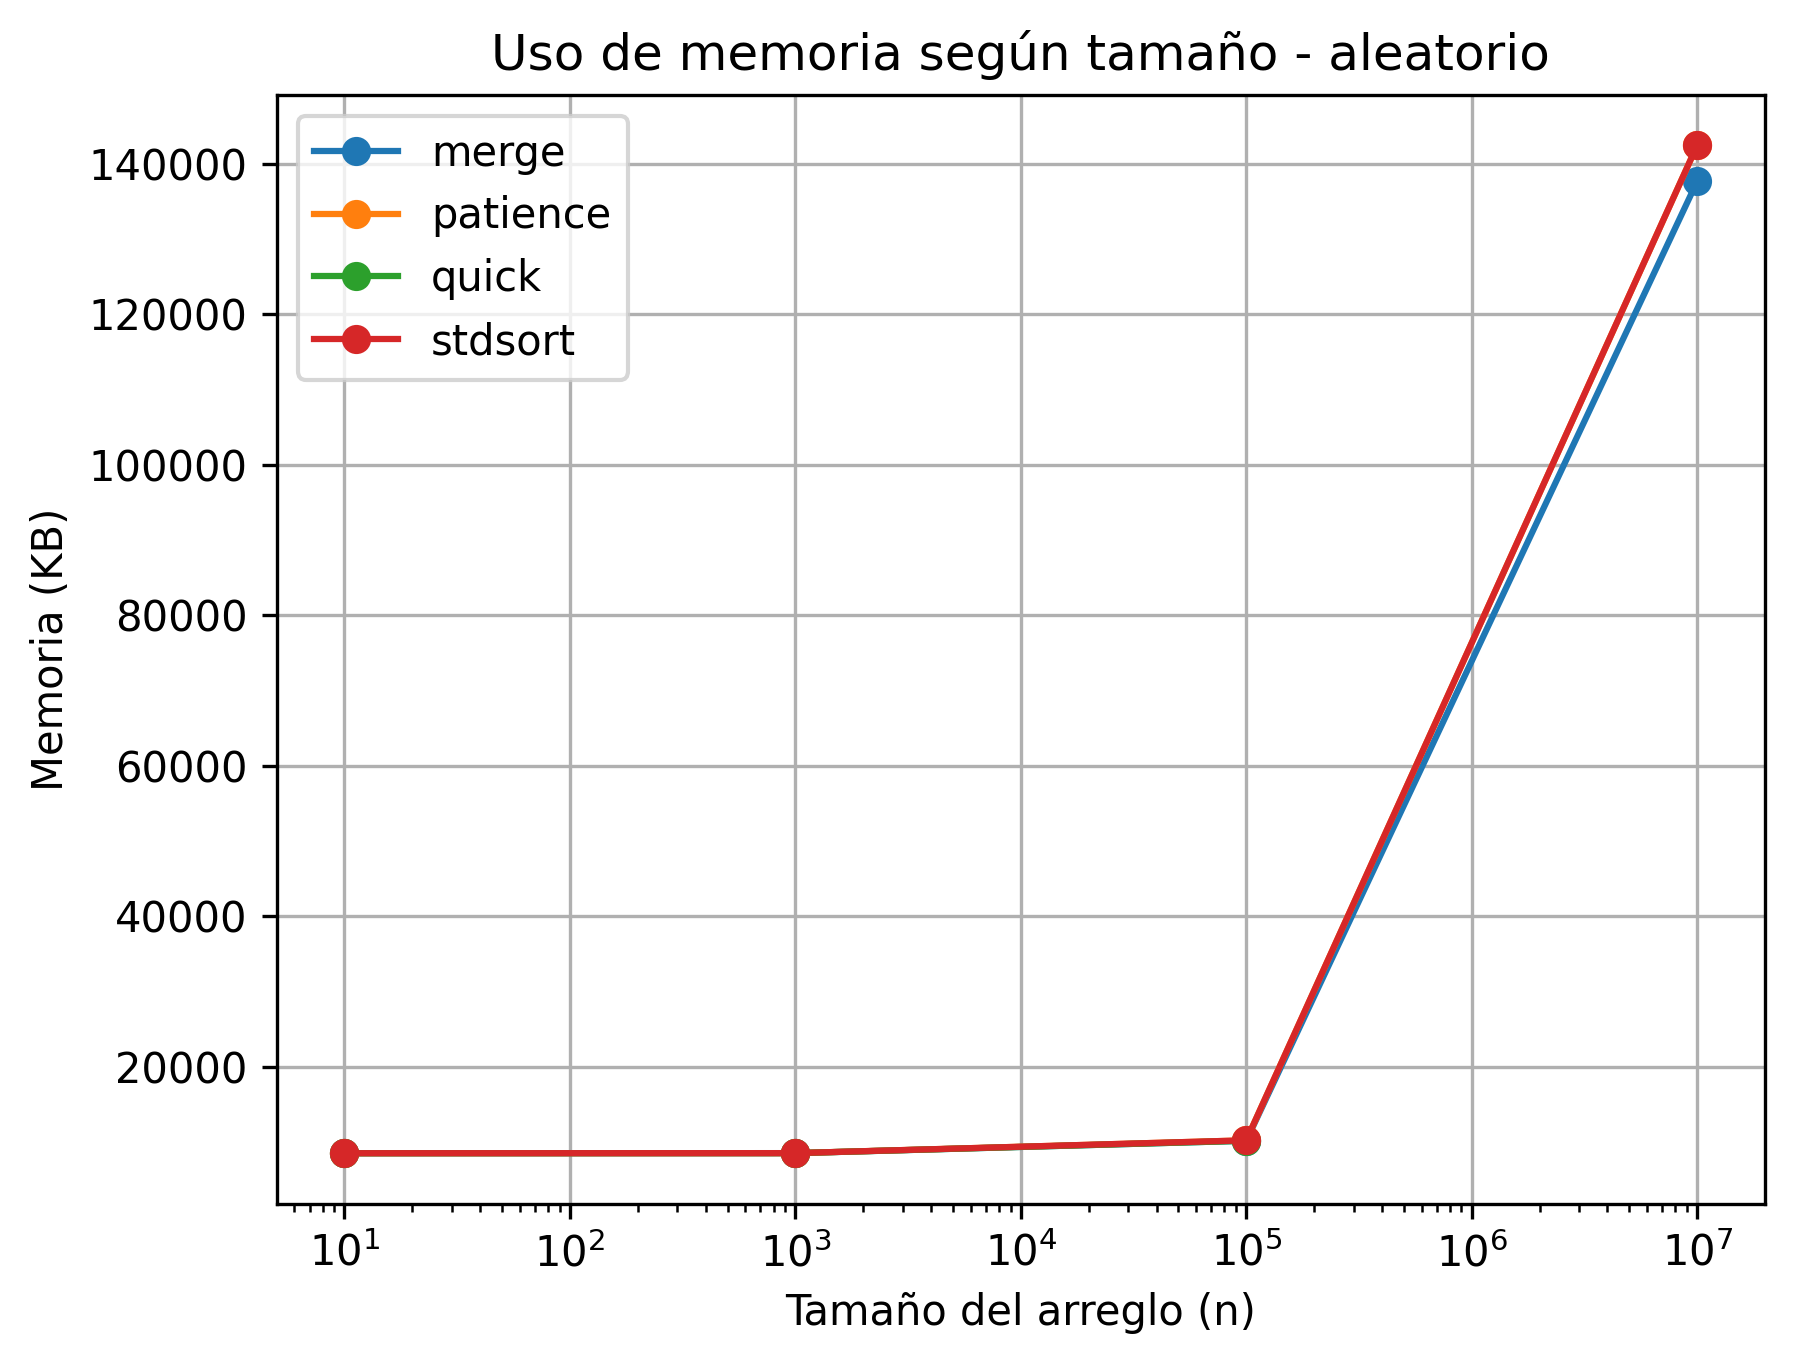
\includegraphics[width=0.45\textwidth]{code/sorting/data/plots/sorting_memoria_vs_n_aleatorio.png}
    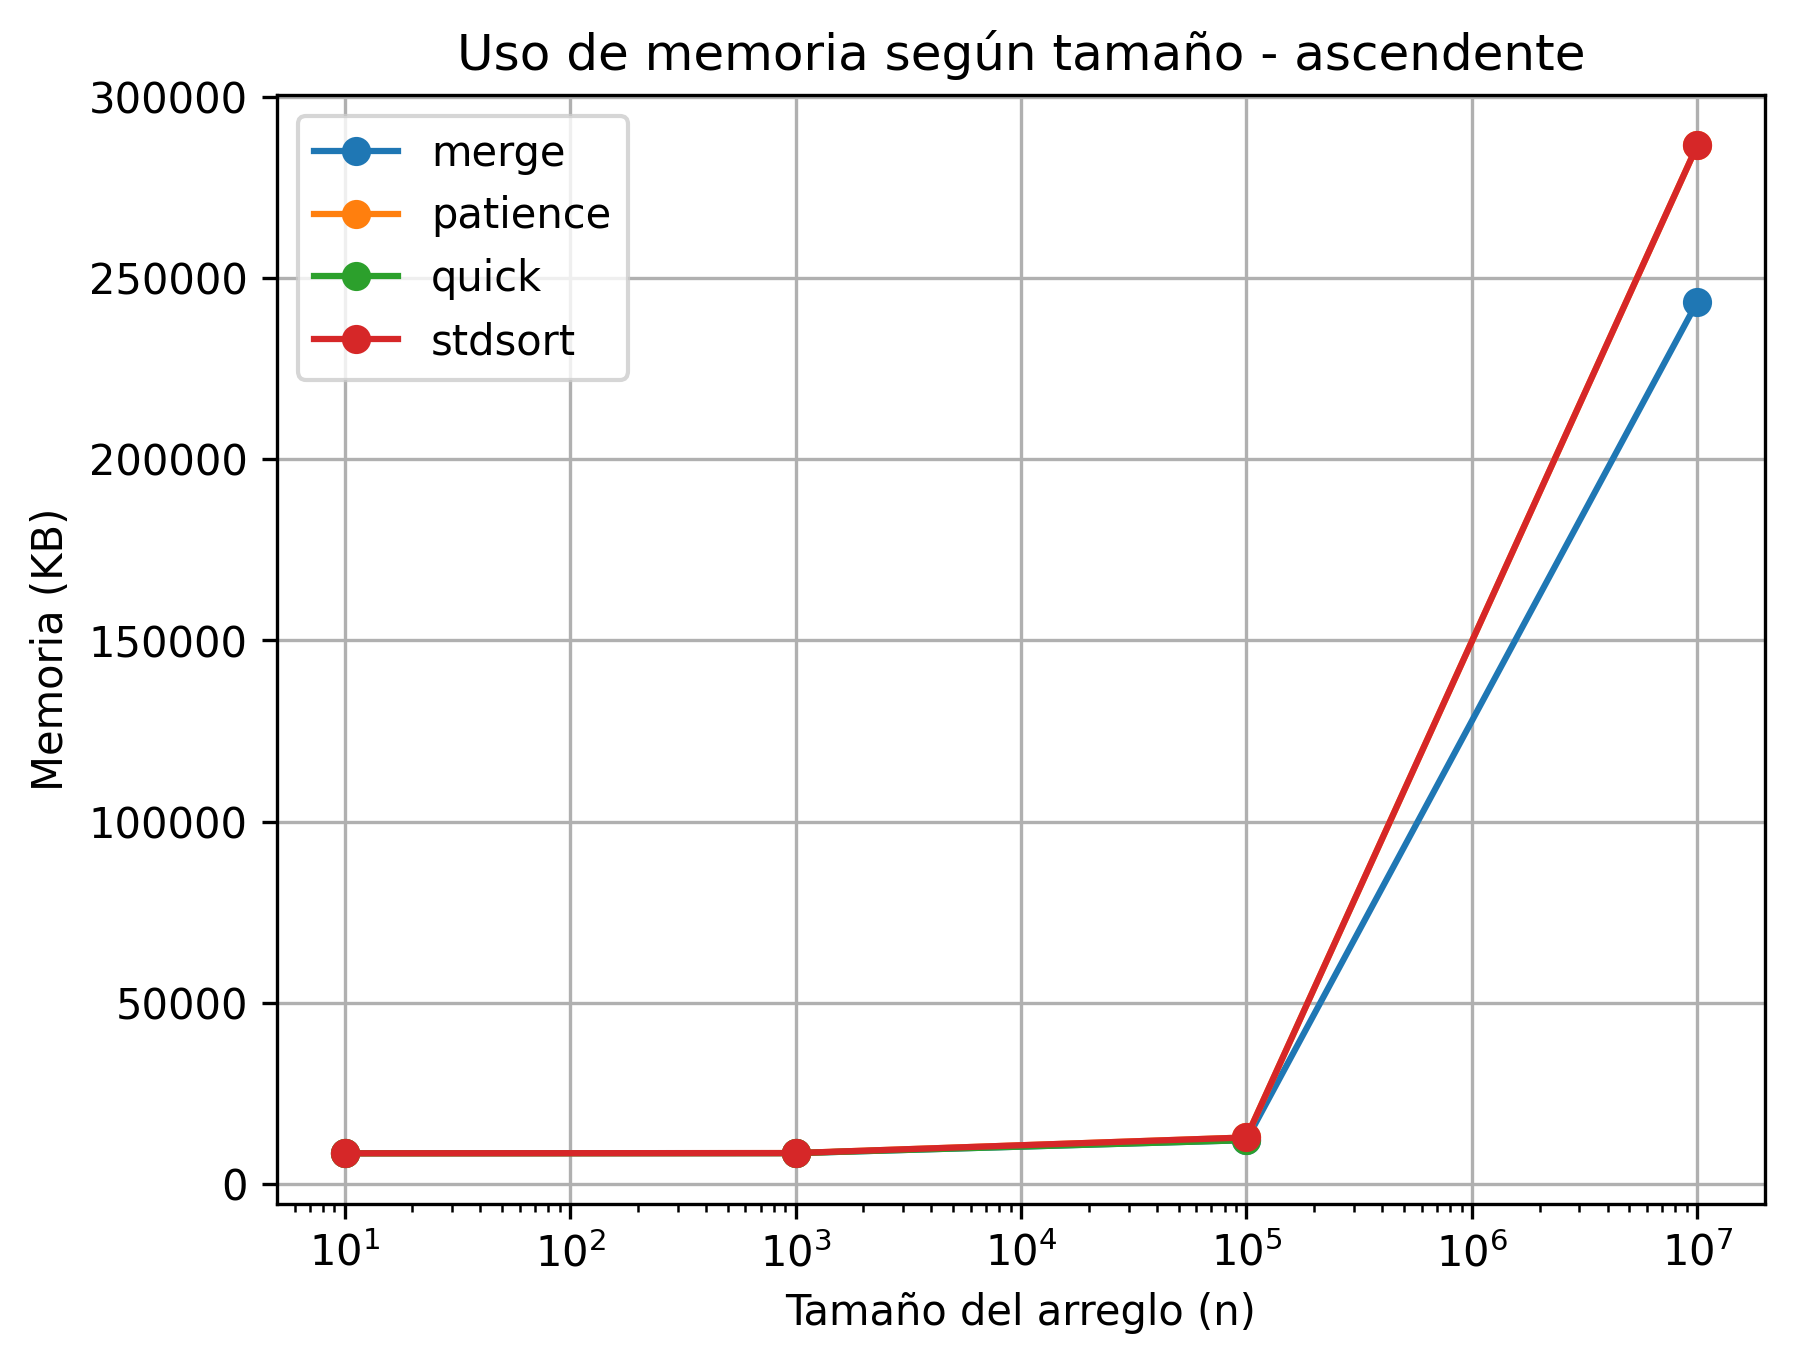
\includegraphics[width=0.45\textwidth]{code/sorting/data/plots/sorting_memoria_vs_n_ascendente.png}
    \caption{Uso de memoria (KB) en arreglos aleatorios (izq.) y ascendentes (der.).}
    \label{fig:app_mem_sorting}
\end{figure}

\subsection*{A.2 Uso de Memoria en Multiplicación de Matrices}
Para las matrices (Figura \ref{fig:app_mem_matrix}), el algoritmo de Strassen requiere consistentemente más memoria que la implementación Naive debido a las asignaciones de submatrices en las llamadas recursivas.

\begin{figure}[H]
    \centering
    
\includegraphics[width=0.45\textwidth]{code/matrix_multiplication/data/plots/memoria_kb_vs_n_densa.png}
    
\includegraphics[width=0.45\textwidth]{code/matrix_multiplication/data/plots/memoria_kb_vs_n_dispersa.png}
    \caption{Uso de memoria (KB) vs $n$ para matrices densas (izq.) y dispersas (der.).}
    \label{fig:app_mem_matrix}
\end{figure}

\subsection*{A.3 Tiempos de Ejecución para Tamaños Estáticos}
Las Figuras \ref{fig:app_time_sort_fixed} y \ref{fig:app_time_matrix_fixed} ilustran el tiempo de ejecución dejando $n$ fijo y variando la naturaleza de los datos. Resulta evidente que la distribución inicial afecta drásticamente a Patience Sort y Quick Sort.

\begin{figure}[H]
    \centering
    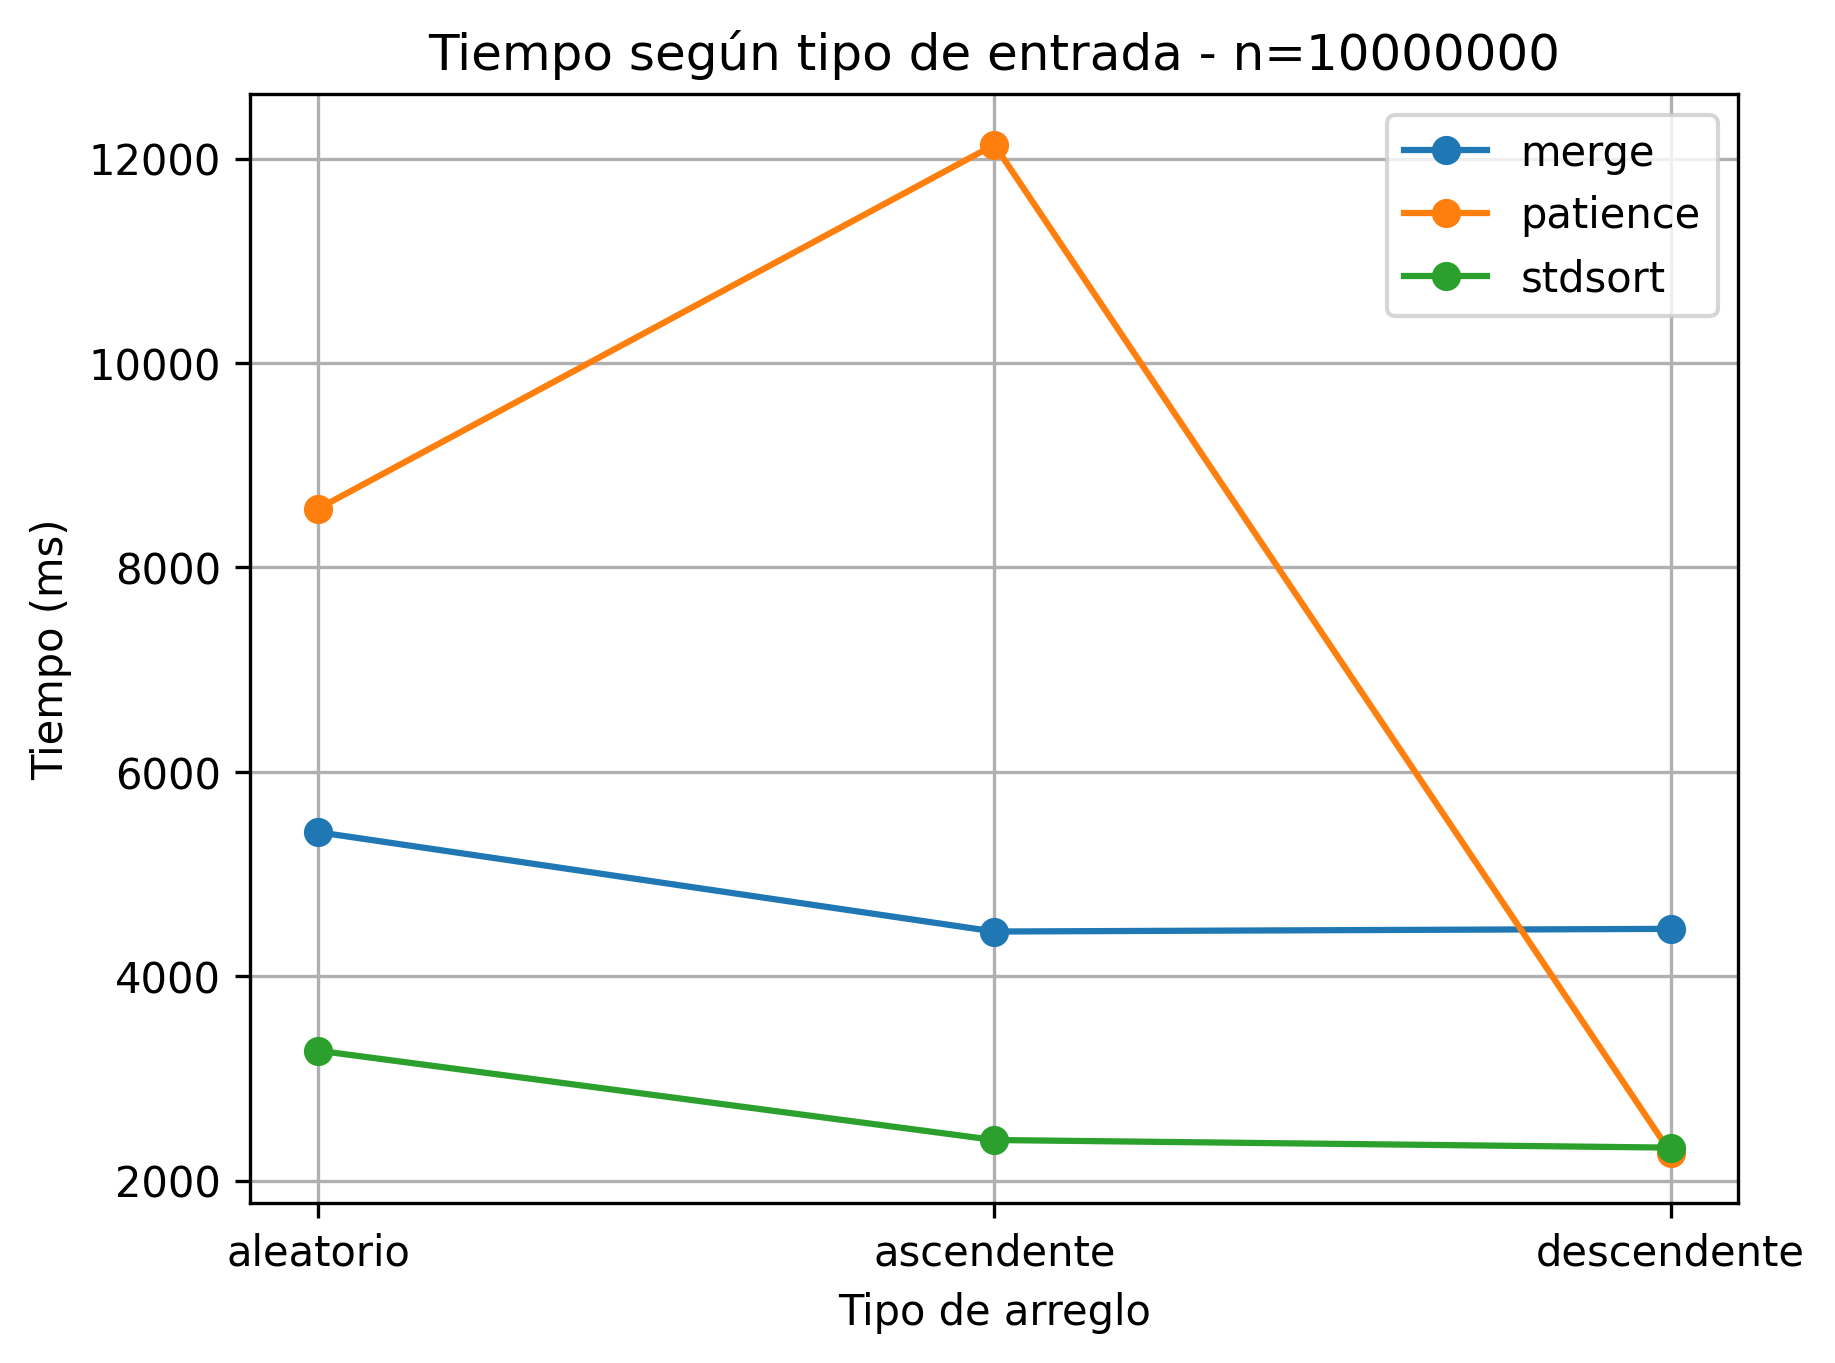
\includegraphics[width=0.45\textwidth]{code/sorting/data/plots/sorting_tiempo_por_tipo_n10000000.png}
    \caption{Tiempos de ordenamiento según tipo de arreglo para el tamaño máximo evaluado ($n=10^7$).}
    \label{fig:app_time_sort_fixed}
\end{figure}

\begin{figure}[H]
    \centering
    
\includegraphics[width=0.45\textwidth]{code/matrix_multiplication/data/plots/tiempo_por_tipo_n256.png}
    \caption{Tiempos de multiplicación según el tipo de matriz para el tamaño máximo evaluado ($n=256$).}
    \label{fig:app_time_matrix_fixed}
\end{figure}


 